\documentclass{template/openetcs_article}
% Use the option "nocc" if the document is not licensed under Creative Commons
%\documentclass[nocc]{template/openetcs_article}
\usepackage{lipsum,url}
\graphicspath{{./template/}{.}{./images/}}
\begin{document}
\frontmatter
\project{openETCS}

%Please do not change anything above this line
%============================
% The document metadata is defined below

%assign a report number here
\reportnum{OETCS/WP4/D4.2-Draft}

%define your workpackage here
\wp{Work-Package 4: ``Verification and Validation''}

%set a title here
\title{Preliminary safety Evaluation Criteria}

%set a subtitle here
\subtitle{Latex Document Draft}

%set the date of the report here
\date{May 2013\\Revised May 2013}

%define a list of authors and their affiliation here

\author{Jan Welte}

\affiliation{Technische Universität Braunschweig\\
  Institute for Traffic Safety and Automation Engineering \\
  Langer Kamp 8 \\
  38118 Braunschweig\\
  Germany}

% define the coverart
\coverart[width=350pt]{openETCS_EUPL}

%define the type of report
\reporttype{Output for secoundary tool evaluation}


\begin{abstract}
%define an abstract here
  This document presents an overview of the safety related evaluation criteria used within the openETCS document structure and based on this derives evaluation criteria for the choice of suitable tools and methods for all safety activities which have to be performed during the openETCS development process. These criteria are based on the safety activities required in D2.6 and the general concept for an openETCS safety process. 
\end{abstract}

%=============================
%Do not change the next three lines
\maketitle
\tableofcontents
\listoffiguresandtables
\newpage
%=============================

% The actual document starts below this line
%=============================


%Start here

\section{Safety Process}



\subsection{Safety artifacts}

Abbreviation	Verification Categorization	Degree of Formalisation
C	Code: used for the executable model	Strictly-Formal
CSB	Code Safety Backlog: list of requirements/ properties to be implemented inside the dM derived from  the HL (and the dMSB)	Semi-Formal/ Strictly-Formal
dM	Detailed Model: model used for code generation	Semi-Formal/ Strictly-Formal
dMSB	Detailed Model Safety Backlog: list of requirements/ properties to be implemented inside the dM derived from the HL (and  the hLSB)	Semi-Formal/ Strictly-Formal
HL	Hazard Log: List of identified hazards and its associated risk classification as well as information concerning the risk control	Informal
hLSB	High Level Safety Backlog: list of requirements/ properties to be implemented inside the hM derived from the HL	Informal/ Semi-Formal
hM	"Higher Model: model derived from srsM or another hM 
and used as an input for dM or another level of hM"	Semi-Formal/ Strictly-Formal
SSHA	Subsystem Hazard Analysis: Safety Analysis of the openETCS subsystem and ist interfaces defined in the SSRS	Informal/ Semi-Formal
Subset-026	Subset 26 version 3.3.0 of the Control Command and Signalling Technical Specification of Interoperability of the trans-European rail system	Informal
Subset-088	Subset-088 version 2.3.0 ETCS Application Levels 1 and 2 - Safety Analysis	Informal/ Semi-Formal
Subset-091	Subset-091 version 3.2.0 Safety Requirements for the Technical Interoperability of ETCS in Levels 1 and 2	Informal
PHA	Preliminary Hazard Analysis of the System, which is mainly delivered based on subset-88 and subset-91	Informal
Safety Goals	General Safety Goal defined for the System mainly related to the accepted level of risk	Informal/ Semi-Formal/Formal
Safety Req	Safety Requirements: list of all requirements which have to be respected during the system development to reach the safety goals	Informal/ Semi-Formal

\subsection{Safety activities}

Abbreviation	System Level Activies	Degree of formalisation
PHA + subset-26->SSHA	Hazard Analysis of the Sub System mainly to identify relevant hazards	Informal -> Informal/Semi-formal
SSHA->HL	Identifying all relevant risks in the subsystem and determining their risk and possible control activities	Informal -> Informal/Semi-formal
HL->SafetyReq	Deriving safety requirements for the subsystem based on all relevant hazards and their associated risk controls  	Informal/Semi-formal -> Informal/Semi-formal
SafetyReq->hLSB	Transformation of all relevant requirements to the level of abstraction of the high level model	Informal/Semi-formal -> Informal/Semi-formal
SafetyReq->dMSB	Transformation of all relevant requirements to the level of abstraction of the detailed Software model	Informal/Semi-formal -> Semi-formal/Strictly-Formal
SafeReq->CSB	Transformation of all relevant requirements to the source code abstraction level	Informal/Semi-formal -> Strictly-Formal
hM/dM/C->HL	Continuous hazard identification during the modelling and model analysis	Informal/Semi-formal -> Informal/Semi-formal
		
Abbreviation	Verification Activities	Degree of formalisation
hM->Safety Req/hLSB	1. Verification of the  higher model against the high level safety requirements	Informal -> Semi-formal/ Strictly-Formal
dM->Safety Req/dMSB	2.  Verification of the  detailed model against the detail safety requirements	Semi-formal/ Strictly-Formal -> Semi-formal/ Strictly-Formal
C->Safety Req/CSB	3. Verification of code against the code safety requirements	Semi-formal/ Strictly-Formal -> Strictly-Formal
		
Abbreviation	Validation Activities	Degree of formalisation
C->HL	1. Validation of the implemented system against all identified hazards and their associated risk	Semi-formal/ Strictly-Formal -> Semi-Formal/ Informal

\begin{figure}[h]
\centering
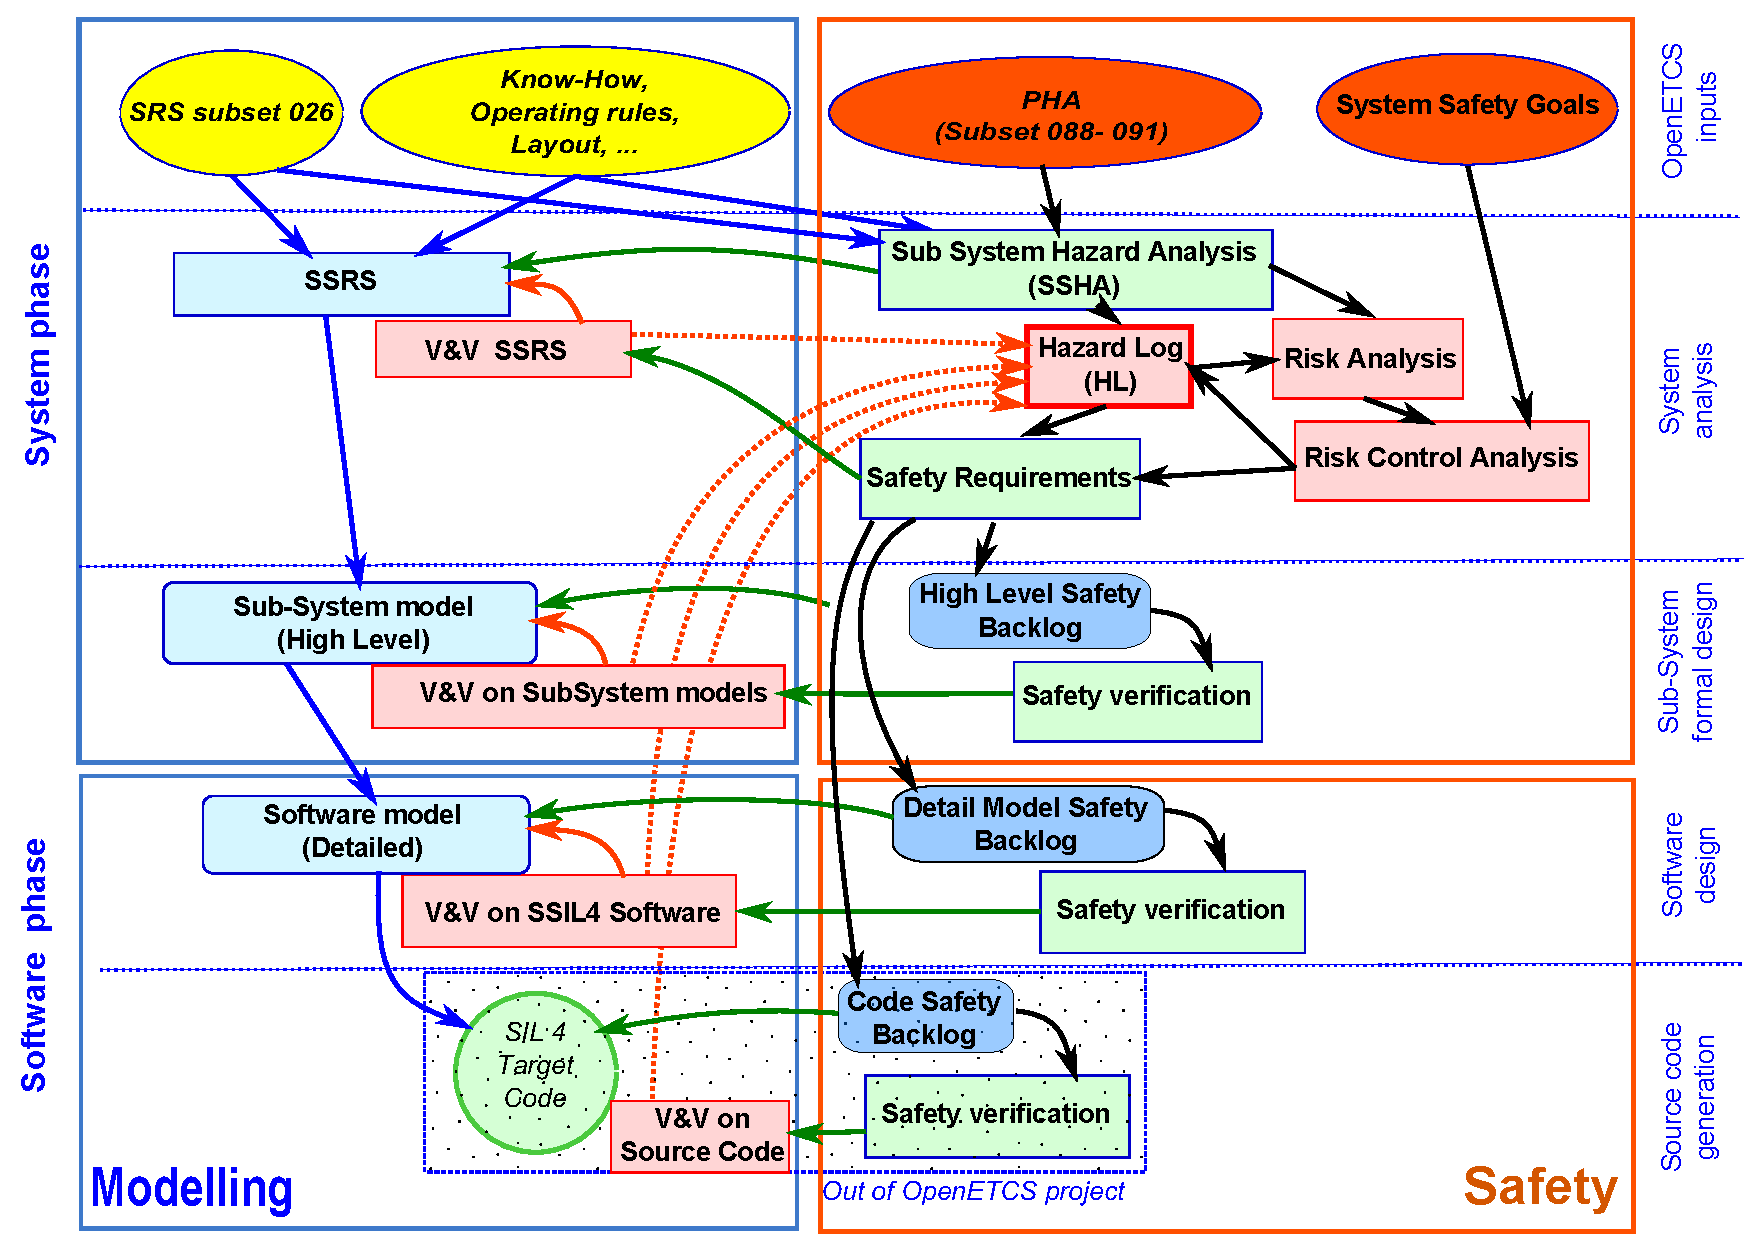
\includegraphics[width=0.8\linewidth]{./images/WholeSafetyProcess}
\caption{OpenETCS Safety Process}
\label{fig:WholeSafetyProcess}
\end{figure}


\subsection{Tools for safety activities}

\section{Evaluation Criteria}

\subsection{Safety artifacts}


\subsection{Safety activities}


\subsection{Tools for safety activities}




\nocite{*}

\bibliographystyle{unsrt}
\bibliography{erdc}



\begin{thebibliography}{9}



\end{thebibliography}

%===================================================
%Do NOT change anything below this line

\end{document}
